\documentclass[9pt,twocolumn,twoside]{styles/osajnl}
\usepackage{fancyvrb}
\journal{i524} 

\title{A Report on Kubernetes}

\author[1]{Srikanth Ramanam}


\affil[1]{School of Informatics and Computing, Bloomington, IN 47408, U.S.A.}


\affil[*]{Corresponding authors: srikrama@iu.edu}

\dates{ \today}

\ociscodes{Cluster, Container, Pod, Kubernetes, I524}



% replace this with your url in github/gitlab
\doi{\url{https://github.com/cloudmesh/classes/blob/master/docs/source/format/report/report.pdf}}

\begin{abstract}
Kubernetes is cluster management software. This paper explores the architecture, functioning and competition of Kubernetes.
\newline
\end{abstract}

\setboolean{displaycopyright}{true}

\begin{document}

\maketitle

\section{Introduction}
Google Kubernetes is a cluster management platform developed by Google. Kubernetes is an open source system for “automating deployment, scaling and management of containerized applications” \cite{www-kubernetesdoc}. It primarily manages clusters through containers as they decouple applications from the host operating system dependencies and allowing their quick and seamless deployment, maintenance and scaling.




\section{About Kubernetes}

Containers gained prominence for their ability to isolate the applications from host operating system dependencies and for being flexible by packaging. Docker tool, that can package applications and their dependencies into containers, was released in 2013, paving way for flexible and portable applications that can run on premises, public and private clouds. Google also decided to release key components of its orchestration, scheduling and load balancing software, called Borg as Open Source. This led to its release in 2015 as Kubernetes \cite{www-kubernetesebook}.



\section{Design}
Kubernetes components are designed to be extensible primarily through Kubernetes API. 
\subsection{Pods}
A pod is a basic unit of Kubernetes scheduling and provides a higher level of abstraction over containers. Pods are collections on containers and resources they are dependent on bundled together. Pods are not durable. They are easily created and deleted as needed.
\subsection{Labels and selectors}
Labels are Key-Value pairs associated with Pods that are queryable. This allows to manage a subset of nodes in a cluster selected through querying on the labels.

\subsection{Services}
A Kubernetes Service is a set of pods usually constitute a tier of an application. Such set of pods are identified by querying their labels. A service usually has an external IP address, a port and a label selector.

\subsection{Controllers}
 These are used for managing for managing the pods. Replication controller replicates specified number of pods to maintain availability. DaemonSet Controller is used for running one pod on each node. And Job Controller is used for running Pods to completion of a task like a batch job.

\section{Architecture}

Kubernetes has a Master-Worker architecture. The worker agents were earlier called minions but are now known as Nodes.
The Kubernetes Master is the controlling unit of the cluster and is responsible for scheduling, managing the workload and communications \cite{www-kubernetesebook}.



\subsection{Master}
\subsubsection{API server}
All the tasks by master and workers are accomplished through API calls, which are handled by API server. This serves the Kubernetes API which provides external and internal interface to Kubernetes API. 
\subsubsection{Etcd}
This is a persistent key-value data store used for storing configuration and overall state of the cluster. Etcd was developed by the CoreOS team.

\subsubsection{Scheduler and Controller Manager}
Controller manager communicates with the API server and creates, manages or deletes pods according to the API calls and/or preset configurations \cite{www-kuberneteswiki}.
\subsection{Worker Node}
\subsubsection{Kubelet}
This is a special background process meant for implementing commands from master. The common commands include create, destroy and monitor its containers.
\subsubsection{Proxy}
This is a network proxy and a load balancer at the node level and is responsible for redirecting the incoming requests to the appropriate containers of the node.
\subsubsection{cAdvisor}
This is an agent that monitors resource usage and performance metrics of containers in nodes.
\section{Functioning}

Usually applications are deployed over clusters as Services which comprise of a collection of pods. We have seen that Pods are groupings of containers and their resources. these services are accessed through the endpoints they expose. Usually the target is to ensure high availability and scalability of services by managing the pods through controllers- creating, allocating and deleting when needed.
\section{User Interface}
Though accessed through API, Kubernetes also provides 
a user interface dashboard providing key metrics.
Figure \ref{fig:ui-dashboard} shows an example figure.

\begin{figure}[htbp]
\centering
\fbox{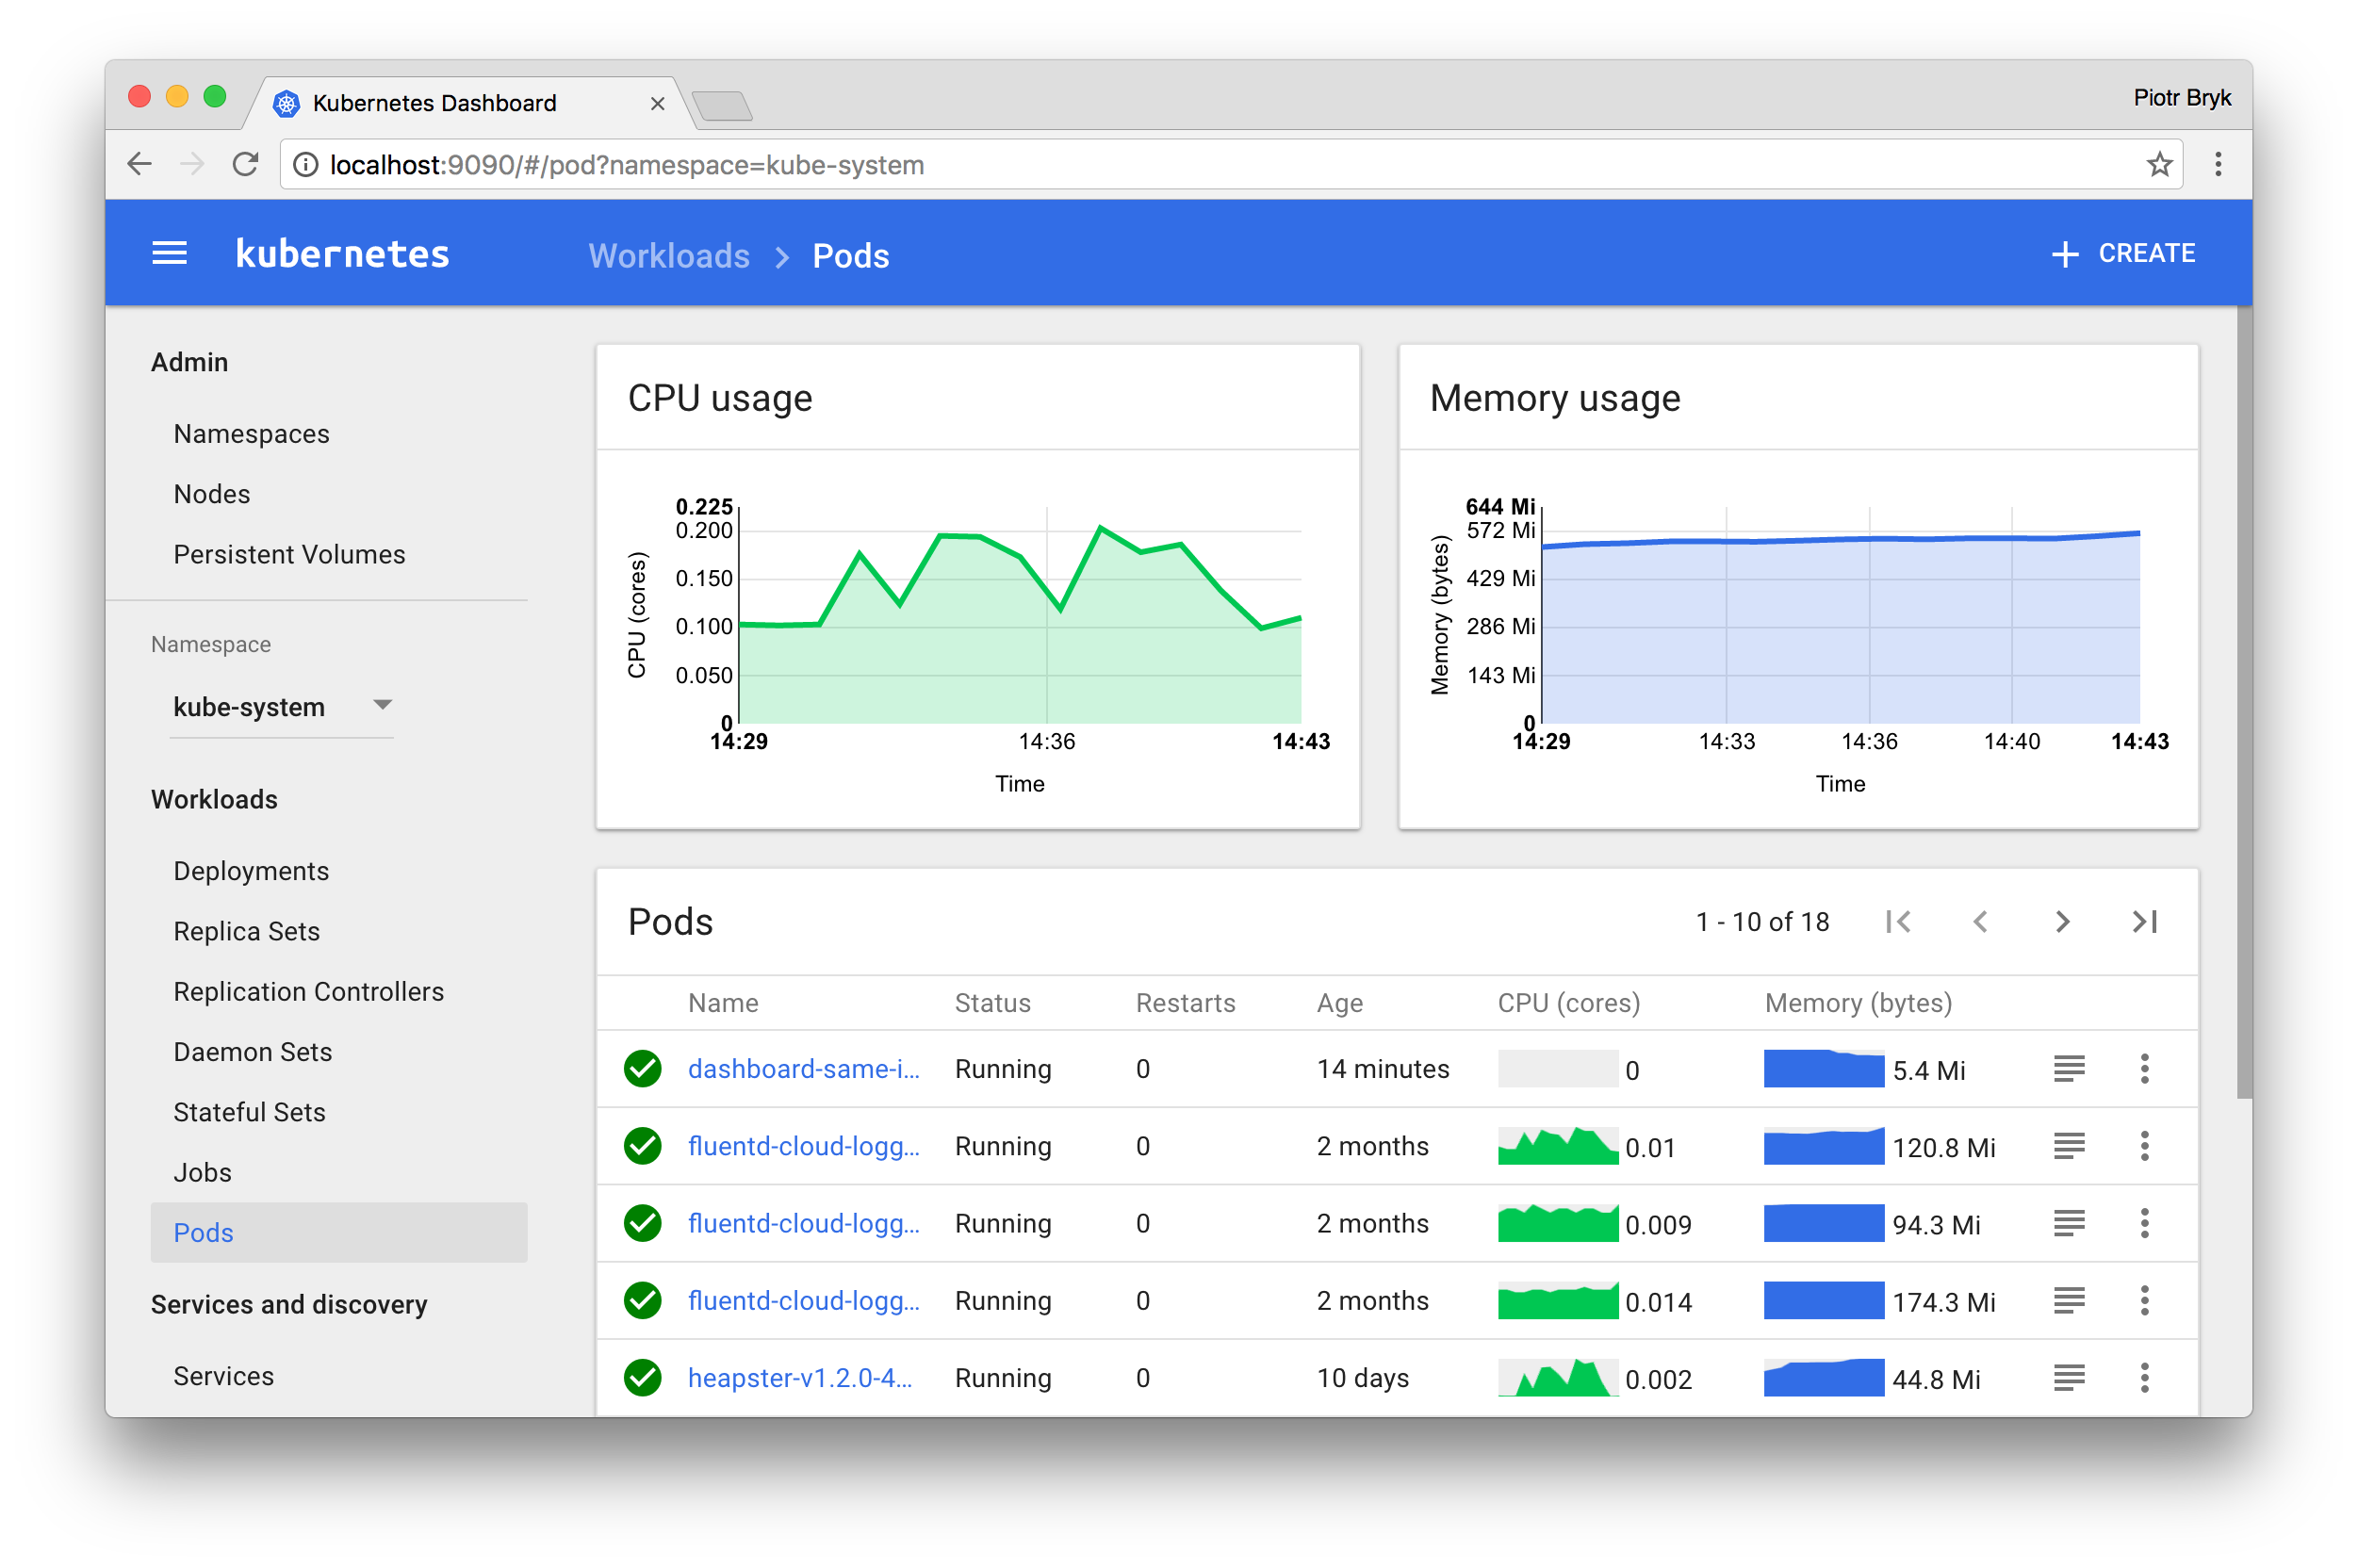
\includegraphics[width=\linewidth]{images/ui-dashboard.png}}
\caption{UI-dashboard \cite{www-kubernetesuidoc}}
\label{fig:Kubernetes UI-dashboard}
\end{figure}
\section{License and Pricing}
Kubernetes is licensed under Apache License 2.0. \cite{www-kuberneteslic}.

\subsection{Pricing}
While Kubernetes itself is free and open source, a paid kubernetes implementation is being offered by Google Cloud Platform.
Nodes are priced between 0.010 USD and 0.240 USD per hour depending on the type of the machine \cite{www-googlecontengpricing}.
0 to 5 node clusters are free when you are paying for the nodes.
6 plus node clusters are being charged at 0.15  USD per hour on top of the price for nodes \cite{www-googlecloudpricing}.
\section{Comparison}
Some of the choices for orchestration, clustering and cluster management are \cite{www-kubernetesarticle}:
\subsection{Docker Swarm}
 Swarm uses the standard  Docker interface. Though this makes it easy to integrate with existing work flows, this may make it difficult to implement complex scheduling with custom interfaces.
\subsection{Fleet}
Fleet is a low level orchestration tool that can be used run other high level orchestration systems such as Kubernetes.
\subsection{Mesos}
Apache Mesos is also a low level, but more stable, scheduler that supports several frameworks for container orchestrations such as Kubernetes, Marathon and Swarm. Usually large applications and in Big Data centers.
\subsection{Kontena}
Kontena a relatively newcomer to the field is aimed at simplifying the whole process and is targeting smaller companies like startups and quicker deployment \cite{www-kontenasite}.
\section{Users}
Some of the Current users of Kubernetes are Pearson, ebay, wikimedia, box, SAP and ComCast \cite{www-kubernetesusers}.
\section{Conclusion}
Kubernetes is an open source custer management software. Kubernetes comes in with the advantage of being the result of 15 years of research and development by Google and is considered stable. It also has an active community of developers. While embracing Kubernetes might involve some redesigning of existing applications, when utilized efficiently it offers a fault-tolerant and efficient system.



\section*{Acknowledgements}

This paper has been written as part of a class assignment for the course: 
I524: Big Data Software and projects, Spring 2017, School of Informatics and computing, Indiana University, Bloomington.
Special thanks to Professor Gregor von Laszewski, Dimitar Nikolov and all associate instructors for guiding through the process of writing this paper.


% Bibliography

\bibliography{references}
 
\end{document}








